\documentclass{book}

\usepackage{titling}
\usepackage{graphicx}
\graphicspath{{.}{assets/}}
\usepackage{microtype}

\usepackage[paperwidth=210mm, paperheight=297mm, textwidth=160mm, textheight=240mm, bindingoffset=1cm]{geometry}

\usepackage[round]{natbib}
\usepackage{hyperref}

\linespread{1.4}
\setlength{\belowcaptionskip}{10pt}

\usepackage{hyphenat}

% Margins.
\usepackage{calc}
\newlength{\lmargin}
\setlength{\lmargin}{1in + \hoffset + \oddsidemargin}

\usepackage{flowfram}
\usepackage{color}
\usepackage{tikz}

% First page column flows are slightly different to the rest.
\newflowframe[1]{7.5cm}{27\baselineskip}{0cm}{0\baselineskip}[firstframe-left]
\newflowframe[1]{7.5cm}{27\baselineskip}{8cm}{0\baselineskip}[firstframe-right]

% Static banner and overlay flow for the first page.
\newstaticframe[1]{\paperwidth}{14cm}{-\lmargin}{12.5cm}[firstframe-banner]
\newstaticframe[1]{14cm}{7\baselineskip}{0cm}{45\baselineskip}[firstframe-overlay]

% Even and odd frame numbering.
\newdynamicframe[odd]{2cm}{2cm}{-\lmargin}{6cm}[numframe-odd]
\newdynamicframe[even]{2cm}{2cm}{\textwidth+\lmargin-2cm}{6cm}[numframe-even]

% The rest of the frames have the same flow.
\newflowframe[>1]{7.5cm}{57\baselineskip}{0cm}{0\baselineskip}[allframes-left]
\newflowframe[>1]{7.5cm}{57\baselineskip}{8cm}{0\baselineskip}[allframes-right]

% Add grey.
\definecolor{grey}{rgb}{0.2, 0.2, 0.2}

% Remove chapter numbering from sections.
\renewcommand*\thesection{\arabic{section}}

\title{Novel Photometry of Bright Stars using Contaminated \textit{Kepler}/K2 Pixels}
\author{Aleksa Sarai}
\date{\today}

\raggedbottom
\begin{document}

\pagestyle{empty}

% Set up page labels.
\begin{dynamiccontents*}{numframe-odd}
	\begin{tikzpicture}
		\draw(0, 0) node [fill=grey, minimum width=2cm, minimum height=2cm]{%
			{\bfseries\Huge\color{white}\thepage}
		};
	\end{tikzpicture}
\end{dynamiccontents*}

\begin{dynamiccontents*}{numframe-even}
	\begin{tikzpicture}
		\draw(0, 0) node [fill=grey, minimum width=2cm, minimum height=2cm]{%
			{\bfseries\Huge\color{white}\thepage}
		};
	\end{tikzpicture}
\end{dynamiccontents*}

\begin{staticcontents*}{firstframe-banner}
	\includegraphics[clip, height=15cm]{kepler.jpg}
\end{staticcontents*}

% Make a pseudo-abstract.
% TODO: Actually make an abstract.
\begin{staticcontents*}{firstframe-overlay}
	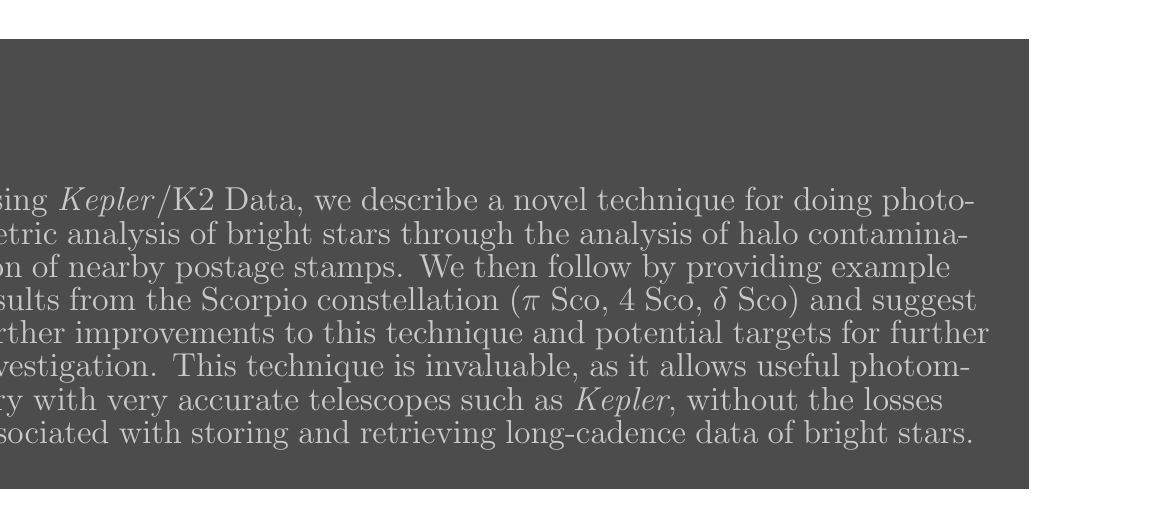
\begin{tikzpicture}
		\draw(0, 0) node [fill=black, text width=13cm, inner sep=5mm, opacity=0.7]{%
			%\sffamily\color{white}
			\color{white}
			\nohyphens{\bfseries\Huge\thetitle}

			\hfill\break
			\nohyphens{\bfseries\it\Large\theauthor}

			\hfill\break
			{\large
				Using \textit{Kepler}/K2 Data, we describe a novel technique for doing
				photometric analysis of bright stars through the analysis of halo
				contamination of nearby postage stamps. We then follow by providing
				example results from the Scorpio constellation ($\pi$ Sco, $4$ Sco,
				$\delta$ Sco) and suggest further improvements to this technique
				and potential targets for further investigation. This technique is
				invaluable, as it allows useful photometry with very accurate telescopes
				such as \textit{Kepler}, without the losses associated with storing
				and retrieving long-cadence data of bright stars.}
		};
	\end{tikzpicture}
\end{staticcontents*}

\section{Background}

\subsection{\textit{Kepler} and K2}

\textit{Kepler} is a space telescope which was sent into space in 2009, and was
at the time one of the most accurate photometric instruments ever sent in to space.
The main benefit was continuous data, allowing for very high time resolution
photometry. \textit{Kepler} orbits the Sun, and made use of 4 reaction wheels to
have very precise pointing control to keep it's intended field of view stationary
on \textit{Kepler}'s detectors \citep{NASA.KEPLER.HANDBOOK}.

The \textit{Kepler} mission has allowed for the discovery of many exoplanets,
and has also allowed for unprecedented astroseismic investigation using
high-precision photometry of many targets. Full technical details for the
\textit{Kepler} telescope can be found in \citet{2010ApJ...713L..87J} and
\citet{2010ApJ...713L..79K}.

However, by 2013 two of the reaction wheels had malfunctioned, rendering the
intended field of view unobservable for continuous periods of time. A second
mission was proposed, K2 \citep{2014PASP..126..398H}. This mission would allow
for \textit{Kepler} to observe new fields despite operating with only two
reaction wheels. However, the observed targets have an apparent motion on the
detectors, as a regular compensation for the rotation of the telescope is done
by using the telescope's thrusters \citep[Section 3]{2013.SHAO.K2}.

During K2, \textit{Kepler} observes along the ecliptic plane, in order for the
solar radiation pressure from the Sun to minimally affect the roll of the spacecraft
\citep{2014PASP..126..398H}. The ecliptic observing field can be seen in \autoref{img:k2fields}.

\begin{staticfigure}
	\centering
		\includegraphics[width=7cm,keepaspectratio]{k2_campaigns}
	\caption{Sequence of observation fields chosen for \textit{Kepler}/K2, all of
			 which lie on the ecliptic plane.}
	\label{img:k2fields}
\end{staticfigure}

\subsubsection{Bandwidth}
\label{section:bandwidth}

Due to \textit{Kepler}'s distance from Earth (and also the immensely large field
of view), the entire field observed cannot be downloaded at high time resolution.
Instead \textit{Kepler} produces ``postage stamps'', which are selections of the
\textit{Kepler} CCD pixels to be downloaded. These pixels are chosen by NASA,
based on proposals by the astronomical community \citep{NASA.PROPOSALS}. An
exposure of the entire \textit{Kepler} field is taken every 30 minutes and the
postage stamps are extracted and saved for download. Every 2 months a
``full frame image'' is also taken, containing all \textit{Kepler} pixels. All
astronomical objects inside or near the \textit{Kepler}/K2 field of view are
assigned a unique identifier known as an ``EPIC target identifier''.

Very bright targets on a \textit{Kepler} CCD cause an effect known as ``bleeding'',
where charge is spilled vertically on the detector, producing a long saturated
streak in one or more columns within the light of the bright star.

\citet{2011MNRAS.411..878K} showed that it is possible to do photometry of bright
targets (specifically, targets which are saturated), but it was generally
believed that this is only possible if \textbf{all} of the flux from the star is
used. One of the main goals of this project was to confirm whether this is indeed
the case.

\subsection{Asteroseismology}

Asteroseismology is the study of stellar oscillations, probing inside stars to
discover their internal structure. This allows for the measurement of stellar
parameters with otherwise unattainable accuracy. While \textit{Kepler} was
primarily an exoplanet finding mission, the high accuracy of its CCD sensors
result in it being the most accurate asteroseismic instrument currently in use.

\subsubsection{Photometry}
\label{section:photometry}

Photometry is a technique that can be used to do asteroseismology. It is, in
essence, counting the amount of photons (flux) that are detected over time. This
time series is then analysed using various techniques to study the oscillations
of the star in question.

%The photons captured are generally only detected if they lie within a certain
%range of frequencies (a bandpass), which result in a skew with regard to the
%detected flux from the star (as a star's black body radiation curve is not uniform
%for all frequencies).

Since the star is not spatially resolved, we can only detect low-degree
oscillations, due to the partial cancellation effect caused by multiple sections
of the star increasing and decreasing in brightness. This can be seen in
\autoref{fig:cancellation}, which quantifies the effect.

\begin{staticfigure}
	\centering
		\includegraphics[width=7cm,keepaspectratio]{cancellation}
	\caption{The partial cancellation factor for photometry for degree $l = 0, \dots, 10$,
			 showing that for degree $l \ge 3$ the cancellation effect renders
			 meaningful photometry very difficult. Reproduced from \citet[Figure 1.5]{2010.ASTEROSEISMOLOGY}}
	\label{fig:cancellation}
\end{staticfigure}

\subsubsection{Bright Stars}

Bright star photometry is very hard, as described in \autoref{section:bandwidth}.
Due to the bandwidth limitation, it is very impractical to download all of the pixels
containing flux from a bright star.

However, bright stars are very important to asteroseismology as they can even be
seen with a rudimentary telescope or the naked eye. As a result, they have been
well studied for hundreds of years, and have accurate distance measurements (as
they are generally closer to earth than other faint stars). Asteroseismic models
are based on several parameters of a star which must be experimentally verified.
By acquiring high-accuracy photometric data for these stars, it is possible to
improve our asteroseismic models of how stars operate. In addition, further
research can be done from the ground.

\section{Method}

The method used in this project was novel, given that standard photometric
techniques of \textit{Kepler}/K2 postage stamps were not applicable to our project.
As such, a large amount of time spent on this project was used to devise and
improve a novel photometric technique, as described below.

\subsection{Halos}

\begin{staticfigure}
	\centering
		\includegraphics[width=7cm,keepaspectratio]{k2_pointspread_large}
	\caption{\textit{Kepler}/K2: A bright star's halo and bleeding column.}
	\label{img:halo}
\end{staticfigure}

Within the \textit{Kepler} telescope, photons can be diffracted and internally
reflected. This is an artefact of how most CCD-based telescope optics operate.
This results in a ghosting effect (as well as diffraction spikes), culminating
in a halo surrounding the star \citep{2009PASP..121.1267S}, as can be seen in
\autoref{img:halo}. The halo is much larger than the actual target, and we
assume it contains a photon count proportional to the main target. This means
that it should be possible (in principle) to do meaningful photometry of a target
using only this halo (and, further, only a subset of the pixels in the halo).

This is a novel idea, and is an improvement to the result by \citet{2011MNRAS.411..878K}
--- that photometry is possible with bright stars using \textit{Kepler} (even if
they cause pixels to be become saturated and produce bleeding columns). Bright
star photometry is a hard problem, as many pixels are saturated as a result of
very bright sources, making it much more expensive in terms of pixels to do
photometry of such targets.

Since pixel bandwidth is very limited, halo photometry could potentially allow
for the study of bright stars without the large number of pixels required for
such studies. However, there is currently no space photometry data for most bright
targets due to the perceived pixel bandwidth requirements. As such, most of the
research done was in trying to find serendipitous postage stamps which contained
halo contamination from a nearby bright star. In that case, it would be possible
to show that halo photometry is viable by masking contaminating halo pixels of
interest.

\subsection{Contamination}

The proposal process of the \textit{Kepler}/K2 mission is not perfect. Not all
postage stamps are checked as thoroughly as possible, so proposals that contain
a large amount of postage stamps may pick postage stamps which are near bright
stars. If a postage stamp is close enough to a bright star, the halo from the
star will contaminate the postage stamp.

\begin{staticfigure}
	\centering
		\includegraphics[width=7cm,keepaspectratio]{k2_contaminated_overlay}
	\caption{\textit{Kepler}/K2: A contaminated postage stamp. Green pixels are
			 the intended target pixels, orange pixels are halo contamination
			 pixels from a nearby bright star.}
	\label{k2:contaminated}
\end{staticfigure}

As can clearly be seen in \autoref{k2:contaminated}, contamination of a bright
star near a postage stamp can be quite significant. This is helped by the intended
EPIC target being very faint in comparison to the halo contamination.

Note that while there may be significant halo contamination in a postage stamp,
not all contamination pixels can be used. Due to the systematics outlined in
\autoref{section:systematics}, some pixels will move out of the postage stamp
rendering them unusable. In addition, the systematics also cause pixels near
bleeding columns to produce an instrumental sawtooth variability.

\subsection{Systematics}
\label{section:systematics}

In order to achieve high precisions, it is important to account for the systematics
of \textit{Kepler}'s motion. Unlike standard \textit{Kepler}/K2 photometry, we
cannot create an aperture around all of the light we wish to capture and ignore
the motion (as done by \citet{2014PASP..126..948V}).

Kepler's systematics are rotational in nature, so a rotational model is required
to digitally track the apparent motion of the contamination in a postage stamp
\citep{2015MNRAS.447.2880A}.

The centroid of each postage stamp on silicon is tracked \citep[p~1784]{2010AJ....139.1782L}
and a rotational model was created. This produces an axis of rotation and
angular velocity for each exposure in a campaign. Using this, it is possible
predict the apparent motion of any set of pixels on silicon with sub-pixel high
accuracy. This invaluable tracking data was provided by Benjamin Pope.

\subsection{Pixel Masks}

As the postage stamp contains a target that we are not interested in, the
pixels whose flux is being integrated over must therefore be chosen based on
whether the pixel is in frame for the campaign (or cadences of interest), the
amount of contamination in a given pixel and that the pixel does not contain
any other sources of variability where possible. Pixel masks were largely chosen
by eye, using the above criteria.

Once a pixel mask has been chosen, a smoothed polygon (or ``aperture'') is
constructed to contain the pixel mask with penumbra smoothing to ensure that
there are minimal edge effects. The aperture is then followed with the apparent
motion of the target, to ensure that the same subsection of the halo is used and
that no brighter or darker regions intrude on the aperture, producing a
systematic variability.

By following the aperture with the apparent motion (which has sub-pixel
accuracy), in principle the same contaminated rays will be captured without
introducing different sources of contamination throughout the analysis.

The amount of flux contained within the aperture is integrated over (fractional
overlap between pixels and the aperture is counted as a weighted sum of the
area of intersection between the pixel boundaries and the aperture), and taken
as the amount of flux in a particular cadence.

\section{Results}

Using the above technique (as well as applications of standard \textit{Kepler}
photometric techniques), several targets were analysed using serendipitous
postage stamp located within the halo of the target.

\subsection{$\pi$ Sco}

\begin{staticfigure}
	\centering
		\includegraphics[width=7cm,keepaspectratio]{pi_sco_aladin}
	\caption{\textit{AladinLite}: Ground-based image of $\pi$ Sco.}
\end{staticfigure}

$\pi$ Sco is an ellipsoidal binary, meaning that there are two stars orbiting
one another. Both stars are elliptical in shape due to tidal forces, so as they
orbit, different surface areas of the star become visible. In addition, the two
stars' transit is on-axis with the Earth so the two stars move in front of one
another over time. This means that the flux from the binary is variable over
time. This binary system has been previously studied, making it a good test to
see if the data obtained from our technique is valid.

\begin{staticfigure}
	\centering
		\includegraphics[width=7cm,keepaspectratio]{pi_203442993_k2overlay}
	\caption{\textit{Kepler}/K2: \texttt{EPIC 203442993}'s postage stamp with
			 all contamination pixels coloured purple, the aperture pixels are
			 coloured purple. Green pixels are the intended EPIC target.}
	\label{img:pi:203442993:mask}
\end{staticfigure}

\texttt{EPIC 203442993} was the chosen postage stamp, and it is clear from
\autoref{img:pi:203442993:mask} that there is plenty of halo contamination present.
A contamination mask with $n = 48$ pixels was chosen to contain all halo pixels
which do not move out of the postage stamp in the time series and also do not
intersect with the bleeding column.

The bleeding column is a completely saturated spike of pixels, however due to
\textit{Kepler}'s rotational systematics, the bleeding column pixels cause an
apparent sawtooth variability. To avoid this, all pixels near the bleeding
column were not included in the halo pixel mask. The chosen mask is overplotted
in \autoref{img:pi:203442993:mask}.

An aperture was constructed using the mask, the aperture was offset to follow
the apparent motion of the contamination for each frame and the flux contained
in the aperture was integrated. The produced light curve then had a high-pass
filter applied with a width of $5 days$ using a $6$th order polynomial. The
Fourier transform of the resulting time series is shown in \autoref{fig:pi:fft}.

\begin{staticfigure}
	\centering
		\includegraphics[width=7cm,keepaspectratio]{pi_sco_lc_k2_fft}
	\caption{Fourier transform of contamination time series. The two peaks near
			 $1~d^{-1}$ are from $\pi$ Sco, and the single peak at $4~d^{-1}$ is
			 due to the motion correction done by Kepler and is entirely
			 instrumental variability.}
	\label{fig:pi:fft}
\end{staticfigure}

We would like to show that the detected variability is not an artefact of our
technique, and is the real variability of $\pi$ Sco. \citet{2005JAD....11....7S}
conducted a photometric study of $\pi$ Sco which used ground-based telescopes
to yield an ellipsoidal period of $1.570103 d$, and provides a phase folded plot
of the flux from the star. This is overplotted in \autoref{fig:pi:both}.

\begin{staticfigure}
	\centering
		\includegraphics[width=7cm,keepaspectratio]{pi_sco_lc_both2}
	\caption{$\pi$ Sco phase folded light curve, comparing halo photometry and
			 \citet{2005JAD....11....7S}.}
	\label{fig:pi:both}
\end{staticfigure}

It is clear that the variability in both lightcurves are identical. This is
proof that the detected variability in using our technique really is from $\pi$
Sco, and that halo photometry is a viable photometric technique. In addition,
\textit{Kepler}/K2 data is far more continuous than ground-based data.

\subsubsection{Ephemeris}

In addition to providing a period, \citet{2005JAD....11....7S} provided the
time of a minima in the signal at some point in the past. This ephemeris can be
used to predict the time of minima in the \textit{Kepler}/K2 data set. This
prediction was used to compute the phase offset in \autoref{fig:pi:both}, which
is definite proof that the detected variability is really from $\pi$ Sco.

\subsection{$4$ Sco}

It is important to ensure that halo photometry does not introduce systematic
variability, and so a bright non-variable star was tested to verify that our
technique is valid.

To this end, the target $4$ Sco was chosen. It is a non-variable star, and
has one nearby postage stamp, \texttt{EPIC 203407633} as can be seen in
\autoref{img:4:203407633}.

\begin{staticfigure}
	\centering
		\includegraphics[width=7cm,keepaspectratio]{4_203407633_k2overlay}
	\caption{\textit{Kepler}/K2: \texttt{EPIC 203407633} -- There is plenty of
			 contamination in the frame. The purple pixels are the selected mask,
			 green are the intended EPIC target and orange are all halo contamination
			 pixels.}
	\label{img:4:203407633}
\end{staticfigure}

It is clear there is significant contamination in the frame. Very similar steps
were taken as with $\pi$ Sco to extract a time series. A Fourier transform is
shown in \autoref{fig:4:fft}, the lack of any distinguishable peak above $3\sigma$
indicates that there is only noise in the contamination. Therefore, our technique
does not add variability which does not exist in the target star, which is a
confirmation of the validity of halo photometry.

\begin{staticfigure}
	\centering
		\includegraphics[width=7cm,keepaspectratio]{4_sco_fft}
	\caption{Fourier transform of contamination time series. There is no clear
			 peak, indicating that the contamination only contains instrumental
			 noise.}
	\label{fig:4:fft}
\end{staticfigure}

\subsection{$\delta$ Sco}
\label{section:delta:results}

$\delta$ Sco is a binary with a highly eccentric, $11$ year orbit \citep{1993AJ...106..7688},
and shows line-profile variability of degree $l = 5 \pm 1$ \citep{1998ASPC..135..149T}.
Photometric confirmation of line-profile variability above $l = 2$ is very
difficult due to the cancellation of high degree spherical oscillations, as
mentioned in \autoref{section:photometry}.

It is possible for $\delta$ Sco to show previously unknown variability, and our
technique could be used to uncover such variability. We found $7$ postage stamps
near $\delta$ Sco which contain halo contamination. None of these postage stamps
have enough useful contaminated pixels. The closest two postage stamps contain
secondary sources of contamination, as in \autoref{img:delta:204367097}.

\begin{staticfigure}
	\centering
		\includegraphics[width=7cm,keepaspectratio]{delta_204367097_k2overlay}
	\caption{\textit{Kepler}/K2: \texttt{EPIC 204367097} -- A secondary source
			 of contamination (blue) is present on the left. Green pixels are the
			 intended EPIC target and orange pixels are the primary source of
			 contamination from $\delta$ Sco}.
	\label{img:delta:204367097}
\end{staticfigure}

As such, many of these postage stamps were rendered unusable. A potential
technique would be to combine the pixels from multiple postage stamps and
doing a weighted sum to use more pixels and perhaps find a signal. However, this
analysis was beyond the scope of this project and could perhaps be followed up
in future research.

\section{Future Research}

The bulk of this project was spent devising and improving the contamination
photometry technique. As a result, there was limited scope for application of
this technique to a large number of stars. However, as this technique has been
shown to be effective, further research can be done into improving halo
photometry and studying bright stars with unprecedented precision.

\subsection{Targets}

Several targets in the Scorpio constellation were studied. Future analysis could
be done on the following targets, all of which have serendipitous postage stamps
within their halo:

\begin{itemize}
	\item $\omega_{1}$ Sco
	\item $i$ Sco
	\item $\nu$ Sco
	\item $\rho$ Oph
\end{itemize}

In addition, campaigns in \textit{Kepler}/K2 other than campaign $2$ (specifically
campaign $4$ which contains the Pleiades cluster) also contain bright stars which
could be surveyed using this technique.

As mentioned in \autoref{section:delta:results}, further research into combining
postage stamps near $\delta$ Sco could lead to the discovery of previously unknown
variability using this technique.

\subsection{\textit{Kepler}/K2 Proposals}

Postage stamps for the \textit{Kepler}/K2 campaigns are chosen based on
community proposals which are approved by NASA. Following on from this research,
it would be plausible to have proposals of postage stamps which contain a subset
of the halo pixels of a bright star to be accepted by the \textit{Kepler}/K2
committee.

This would allow high-precision photometry of all of the pixels in a postage
stamp for halo photometry, without the need to mask out pixels which are
rendered useless due an unrelated EPIC target being in the postage stamp.

\section{Conclusion}

We have shown that halo photometry is a viable technique for the study of bright
stars which could not have been studied previously, without downloading large
amounts of pixels. Several stars were studied, and some other stars were proposed
for future studies. The research undertaken as part of this project has resulted
in an entirely new method of doing photometry with \textit{Kepler}/K2 data, with
potential applications to other space photometry data.

\section{Acknowledgements}

I would like to thank Tim Bedding, Daniel Huber and Simon Murphy for their
invaluable help as my supervisors. In addition, the data and advice given by
Benjamin Pope and Tim White was also invaluable.

In addition, the \textit{Kepler} team and NASA should be acknowledged for
making all of the \textit{Kepler}/K2 data publicly available.

And, finally, I would like to thank Helen Johnston for organising the Talented
Student Program and allowing me the opportunity to carry out this project.

\let\cleardoublepage\clearpage

{\footnotesize
\bibliographystyle{plainnat}
\renewcommand\bibname{\Large References}
\bibliography{references}}

\end{document}
